% Generated 2019-05-29 09:29:21 -0400
\subsection{Assets} \label{model:Assets}
\subsubsection{Defintion of \texttt{ MTAssetType}}
  \label{type:MTAssetType}

\FloatBarrier

An Asset is a container type XML element used to organize information describing an 
entity that is not a piece of equipment.  Asset is an abstract type and will never 
appear directly in the MTConnect information model.

\begin{table}[ht]
\centering 
  \caption{\texttt{MTAssetType} Definition}
  \label{table:MTAssetType}
\fontsize{9pt}{11pt}\selectfont
\tabulinesep=3pt
\begin{tabu} to 6in {|X[-1.35]|X[-0.7]|X[-1.75]|X[-1.5]|X[-1]|X[-0.7]|} \everyrow{\hline}
\hline
\rowfont\bfseries {Attribute} & \multicolumn{5}{|l|}{Value} \\
\tabucline[1.5pt]{}
BrowseName & \multicolumn{5}{|l|}{MTAssetType} \\
IsAbstract & \multicolumn{5}{|l|}{True} \\
\tabucline[1.5pt]{}
\rowfont \bfseries References & NodeClass & BrowseName & DataType & Type\-Definition & {Modeling\-Rule} \\
\multicolumn{6}{|l|}{Subtype of BaseObjectType (See \cite{UAPart5} Documentation)} \\
HasSubtype & ObjectType & \multicolumn{2}{l}{MTCuttingToolArchetypeType} & \multicolumn{2}{|l|}{See section \ref{type:MTCuttingToolArchetypeType}} \\
HasSubtype & ObjectType & \multicolumn{2}{l}{MTCuttingToolType} & \multicolumn{2}{|l|}{See section \ref{type:MTCuttingToolType}} \\
Has\-Property & Variable & Asset\-Id & String & Property\-Type & Mandatory \\
Has\-Property & Variable & Device\-Uuid & String & Property\-Type & Mandatory \\
Has\-Property & Variable & MT\-Description & String & Property\-Type & Optional \\
Has\-Property & Variable & Removed & Boolean & Property\-Type & Optional \\
Has\-Property & Variable & Timestamp & Date\-Time & Property\-Type & Mandatory \\
\end{tabu}
\end{table} 


\FloatBarrier
\subsection{Cutting Tool} \label{model:CuttingTool}

\begin{figure}[ht]
  \centering
    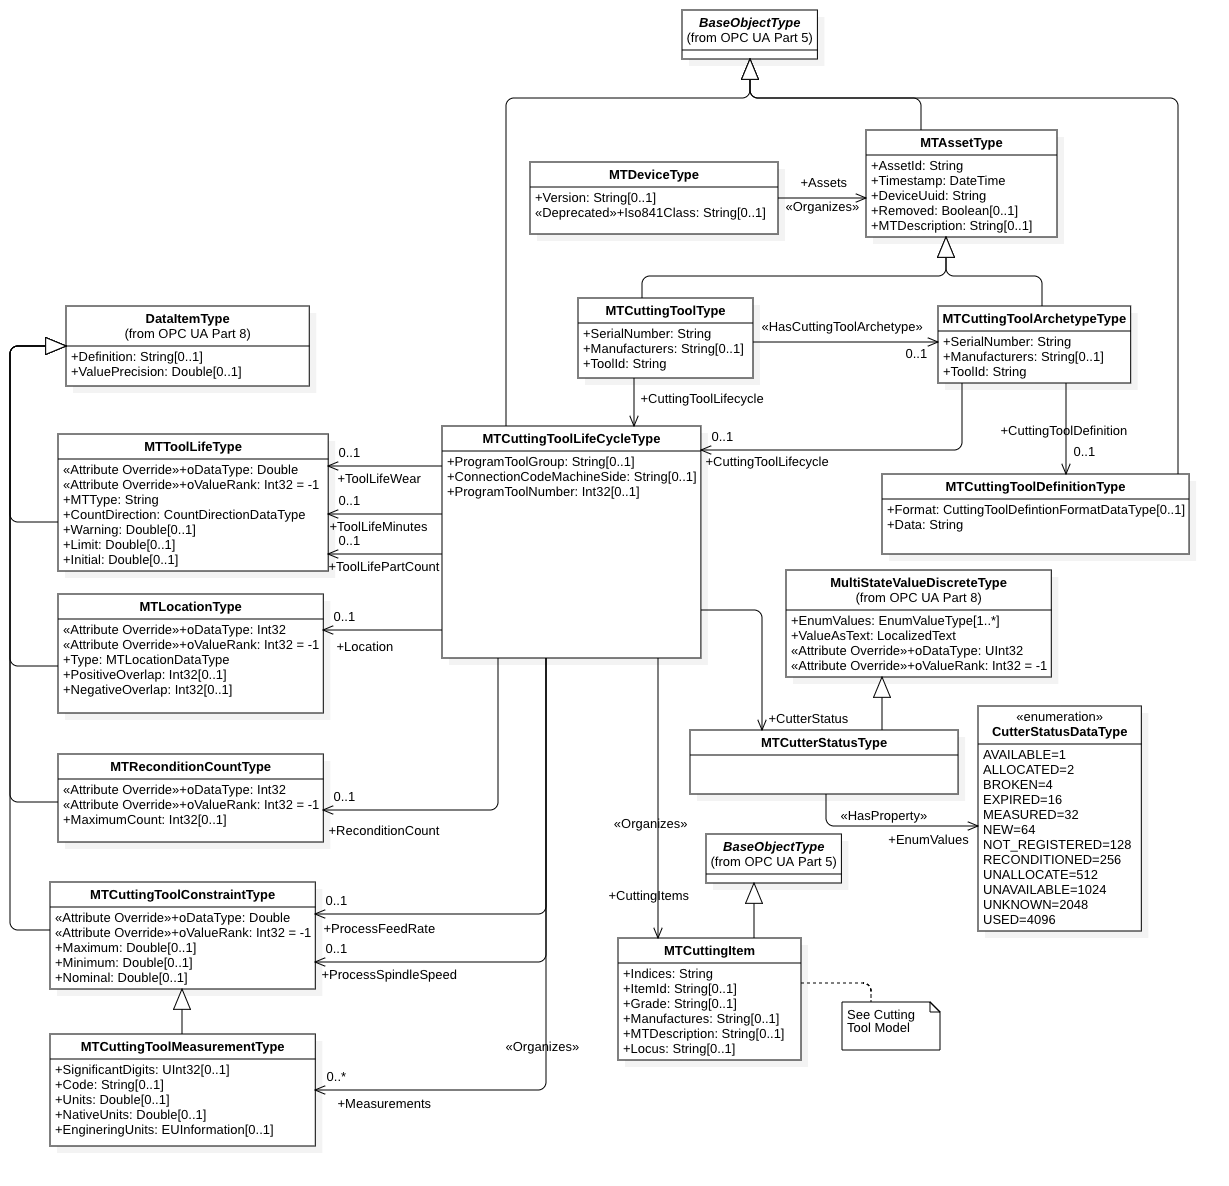
\includegraphics[width=1.0\textwidth]{./diagrams/types/CuttingTool.png}
  \caption{Cutting Tool Diagram}
  \label{fig:CuttingTool}
\end{figure}

\FloatBarrier

\subsubsection{Defintion of \texttt{ MTCutterStatusType}}
  \label{type:MTCutterStatusType}

\FloatBarrier

The values CutterStatus element can be a combined set of Status elements.  The MTConnect Standard allows 
any set of statuses to be combined, but only certain combinations make sense.  A Cutting Tool \shouldnot be 
both \mtmodel{NEW} and \mtmodel{USED} at the same time.  There are no rules in the schema to enforce this, but this 
is left to the implementer. The following combinations \mustnot occur: 

\begin{itemize}
  \item \mtmodel{NEW} \mustnot be used with \mtmodel{USED}, \mtmodel{RECONDITIONED}, or \mtmodel{EXPIRED}. 
  \item \mtmodel{UNKNOWN} \mustnot be used with any other status. 
  \item \mtmodel{ALLOCATED} and \mtmodel{UNALLOCATED} \mustnot be used together.
  \item \mtmodel{AVAILABLE} and \mtmodel{UNAVAILABLE} \mustnot be used together.
  \item If the tool is \mtmodel{EXPIRED}, \mtmodel{BROKEN}, or \mtmodel{NOT_REGISTERED} it \mustnot be \mtmodel{AVAILABLE}.
  \item All other combinations are allowed.
\end{itemize}

\begin{table}[ht]
\centering 
  \caption{\texttt{MTCutterStatusType} Definition}
  \label{table:MTCutterStatusType}
\fontsize{9pt}{11pt}\selectfont
\tabulinesep=3pt
\begin{tabu} to 6in {|X[-1.35]|X[-0.7]|X[-1.75]|X[-1.5]|X[-1]|X[-0.7]|} \everyrow{\hline}
\hline
\rowfont\bfseries {Attribute} & \multicolumn{5}{|l|}{Value} \\
\tabucline[1.5pt]{}
BrowseName & \multicolumn{5}{|l|}{MTCutterStatusType} \\
IsAbstract & \multicolumn{5}{|l|}{False} \\
ValueRank & \multicolumn{5}{|l|}{-2} \\
DataType & \multicolumn{5}{|l|}{UInteger} \\
\tabucline[1.5pt]{}
\rowfont \bfseries References & NodeClass & BrowseName & DataType & Type\-Definition & {Modeling\-Rule} \\
\multicolumn{6}{|l|}{Subtype of MultiStateDiscreteType (See \cite{UAPart8} Documentation)} \\
Has\-Component & Variable & Enum\-Values & Cutter\-Status\-Data\-Type & Cutter\-Status\-Data\-Type & Mandatory \\
\end{tabu}
\end{table} 


\FloatBarrier
\paragraph{Referenced Properties and Objects}

\begin{itemize}
\item \textbf{Allowable Values} for \texttt{CutterStatusDataType}
\FloatBarrier
\begin{table}[ht]
\centering 
  \caption{\texttt{CutterStatusDataType} Enumeration}
  \label{enum:CutterStatusDataType}
\tabulinesep=3pt
\begin{tabu} to 6in {|l|r|} \everyrow{\hline}
\hline
\rowfont\bfseries {Name} & {Index} \\
\tabucline[1.5pt]{}
\texttt{AVAILABLE} & \texttt{1} \\
\texttt{ALLOCATED} & \texttt{2} \\
\texttt{BROKEN} & \texttt{4} \\
\texttt{EXPIRED} & \texttt{16} \\
\texttt{MEASURED} & \texttt{32} \\
\texttt{NEW} & \texttt{64} \\
\texttt{NOT_REGISTERED} & \texttt{128} \\
\texttt{RECONDITIONED} & \texttt{256} \\
\texttt{UNALLOCATE} & \texttt{512} \\
\texttt{UNAVAILABLE} & \texttt{1024} \\
\texttt{UNKNOWN} & \texttt{2048} \\
\texttt{USED} & \texttt{4096} \\
\end{tabu}
\end{table} 
\FloatBarrier
\end{itemize}
\FloatBarrier
\subsubsection{Defintion of \texttt{ MTCuttingItemType}}
  \label{type:MTCuttingItemType}

\FloatBarrier

\begin{figure}[ht]
  \centering
    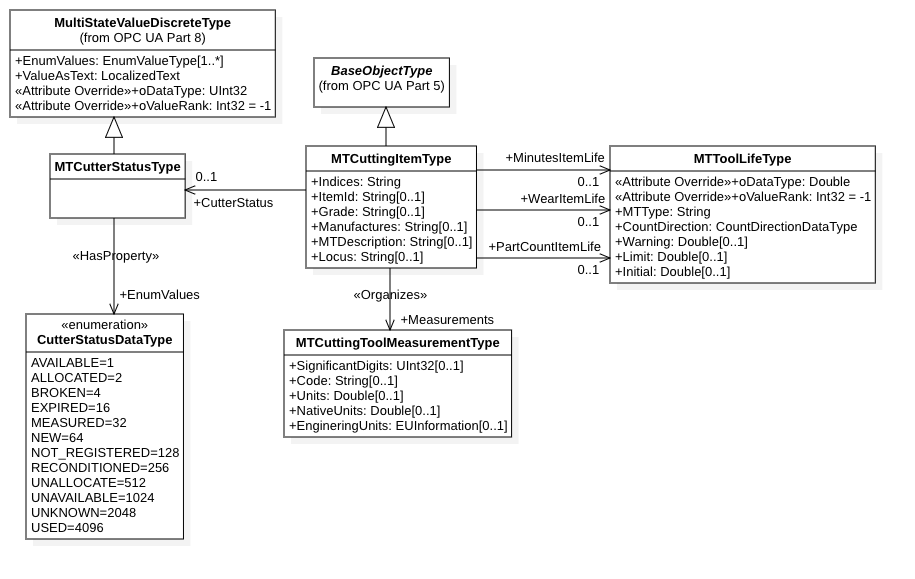
\includegraphics[width=1.0\textwidth]{./diagrams/types/MTCuttingItemType.png}
  \caption{MTCuttingItemType Diagram}
  \label{fig:MTCuttingItemType}
\end{figure}

\FloatBarrier

\begin{table}[ht]
\centering 
  \caption{\texttt{MTCuttingItemType} Definition}
  \label{table:MTCuttingItemType}
\fontsize{9pt}{11pt}\selectfont
\tabulinesep=3pt
\begin{tabu} to 6in {|X[-1.35]|X[-0.7]|X[-1.75]|X[-1.5]|X[-1]|X[-0.7]|} \everyrow{\hline}
\hline
\rowfont\bfseries {Attribute} & \multicolumn{5}{|l|}{Value} \\
\tabucline[1.5pt]{}
BrowseName & \multicolumn{5}{|l|}{MTCuttingItemType} \\
IsAbstract & \multicolumn{5}{|l|}{False} \\
\tabucline[1.5pt]{}
\rowfont \bfseries References & NodeClass & BrowseName & DataType & Type\-Definition & {Modeling\-Rule} \\
\multicolumn{6}{|l|}{Subtype of BaseObjectType (See \cite{UAPart5} Documentation)} \\
Has\-Property & Variable & Grade & String & Property\-Type & Optional \\
Has\-Property & Variable & Indices & String & Property\-Type & Mandatory \\
Has\-Property & Variable & Item\-Id & String & Property\-Type & Optional \\
Has\-Property & Variable & Locus & String & Property\-Type & Optional \\
Has\-Property & Variable & Manufactures & String[] & Property\-Type & Optional \\
Has\-Property & Variable & MT\-Description & String & Property\-Type & Optional \\
Has\-Component & Variable & Minutes\-Item\-Life & Base\-Data\-Type & MT\-Tool\-Life\-Type & Optional \\
Has\-Component & Variable & Cutter\-Status & UInteger & MT\-Cutter\-Status\-Type & Optional \\
Has\-Component & Variable & Part\-Count\-Item\-Life & Base\-Data\-Type & MT\-Tool\-Life\-Type & Optional \\
Organizes & Object & <Folder> & MT\-Cutting\-Tool\-Measurement\-Type[] & Folder\-Type & Optional \\
Has\-Component & Variable & Wear\-Item\-Life & Base\-Data\-Type & MT\-Tool\-Life\-Type & Optional \\
\end{tabu}
\end{table} 


\FloatBarrier
\paragraph{Referenced Properties and Objects}

\begin{itemize}
\item \texttt{Indices::String:} TODO: We may want to create a special type for the indices.

\end{itemize}
\FloatBarrier
\subsubsection{Defintion of \texttt{ MTCuttingItemsFolderType}}
  \label{type:MTCuttingItemsFolderType}

\FloatBarrier
\begin{table}[ht]
\centering 
  \caption{\texttt{MTCuttingItemsFolderType} Definition}
  \label{table:MTCuttingItemsFolderType}
\fontsize{9pt}{11pt}\selectfont
\tabulinesep=3pt
\begin{tabu} to 6in {|X[-1.35]|X[-0.7]|X[-1.75]|X[-1.5]|X[-1]|X[-0.7]|} \everyrow{\hline}
\hline
\rowfont\bfseries {Attribute} & \multicolumn{5}{|l|}{Value} \\
\tabucline[1.5pt]{}
BrowseName & \multicolumn{5}{|l|}{MTCuttingItemsFolderType} \\
IsAbstract & \multicolumn{5}{|l|}{False} \\
\tabucline[1.5pt]{}
\rowfont \bfseries References & NodeClass & BrowseName & DataType & Type\-Definition & {Modeling\-Rule} \\
\multicolumn{6}{|l|}{Subtype of FolderType (See \cite{UAPart5} Documentation)} \\
Has\-Property & Variable & Count & Int32 & Property\-Type & Mandatory \\
Organizes & Object & <Folder> & MT\-Cutting\-Tool\-Life\-Cycle\-Type & Folder\-Type & Mandatory \\
\end{tabu}
\end{table} 


\FloatBarrier
\subsubsection{Defintion of \texttt{ MTCuttingItemsFolderType}}
  \label{type:MTCuttingItemsFolderType}

\FloatBarrier
\begin{table}[ht]
\centering 
  \caption{\texttt{MTCuttingItemsFolderType} Definition}
  \label{table:MTCuttingItemsFolderType}
\fontsize{9pt}{11pt}\selectfont
\tabulinesep=3pt
\begin{tabu} to 6in {|X[-1.35]|X[-0.7]|X[-1.75]|X[-1.5]|X[-1]|X[-0.7]|} \everyrow{\hline}
\hline
\rowfont\bfseries {Attribute} & \multicolumn{5}{|l|}{Value} \\
\tabucline[1.5pt]{}
BrowseName & \multicolumn{5}{|l|}{MTCuttingItemsFolderType} \\
IsAbstract & \multicolumn{5}{|l|}{False} \\
\tabucline[1.5pt]{}
\rowfont \bfseries References & NodeClass & BrowseName & DataType & Type\-Definition & {Modeling\-Rule} \\
Has\-Property & Variable & Count & Int32 & Property\-Type & Mandatory \\
\end{tabu}
\end{table} 


\FloatBarrier
\subsubsection{Defintion of \texttt{ MTCuttingToolArchetypeType}}
  \label{type:MTCuttingToolArchetypeType}

\FloatBarrier

The \mtuatype{MTCuttingToolArchetypeType} \mtterm{Information Model} represents the information about
a of cutting tool that is common to all cutting toos of that kind. It contains only the constraints
on the measurements and the limits of use, but as it deos not represent a physical cutting tool, there
can be not measured values.
 

MTConnect Standard will adopt the ISO 13399 structure when formulating the vocabulary 
for Cutting Tool geometries and structure to be represented in the CuttingToolArchetype.  
The nominal values provided in the \mtuatype{MTCuttingToolLifeCycleType} section are only concerned with two 
aspects of the Cutting Tool, the Cutting Tool and the Cutting Item.  The Tool Item, Adaptive 
Item, and Assembly Item will only be covered in the \mtuatype{MTCuttingToolDefinitionType} section of this 
document since this section contains the full ISO 13399 information about a Cutting Tool.

\begin{table}[ht]
\centering 
  \caption{\texttt{MTCuttingToolArchetypeType} Definition}
  \label{table:MTCuttingToolArchetypeType}
\fontsize{9pt}{11pt}\selectfont
\tabulinesep=3pt
\begin{tabu} to 6in {|X[-1.35]|X[-0.7]|X[-1.75]|X[-1.5]|X[-1]|X[-0.7]|} \everyrow{\hline}
\hline
\rowfont\bfseries {Attribute} & \multicolumn{5}{|l|}{Value} \\
\tabucline[1.5pt]{}
BrowseName & \multicolumn{5}{|l|}{MTCuttingToolArchetypeType} \\
IsAbstract & \multicolumn{5}{|l|}{False} \\
\tabucline[1.5pt]{}
\rowfont \bfseries References & NodeClass & BrowseName & DataType & Type\-Definition & {Modeling\-Rule} \\
\multicolumn{6}{|l|}{Subtype of MTAssetType (See Assets Documentation)} \\
Has\-Property & Variable & Manufacturers & String[] & Property\-Type & Optional \\
Has\-Property & Variable & Serial\-Number & String & Property\-Type & Mandatory \\
Has\-Property & Variable & Tool\-Id & String & Property\-Type & Mandatory \\
Has\-Component & Object & Cutting\-Tool\-Lifecycle & \multicolumn{2}{l|}{MTCuttingToolLifeCycleType} & Optional \\
Has\-Component & Object & Cutting\-Tool\-Definition & \multicolumn{2}{l|}{MTCuttingToolDefinitionType} & Optional \\
\end{tabu}
\end{table} 


\FloatBarrier
\subsubsection{Defintion of \texttt{ MTCuttingToolConstraintType}}
  \label{type:MTCuttingToolConstraintType}

\FloatBarrier
\begin{table}[ht]
\centering 
  \caption{\texttt{MTCuttingToolConstraintType} Definition}
  \label{table:MTCuttingToolConstraintType}
\fontsize{9pt}{11pt}\selectfont
\tabulinesep=3pt
\begin{tabu} to 6in {|X[-1.35]|X[-0.7]|X[-1.75]|X[-1.5]|X[-1]|X[-0.7]|} \everyrow{\hline}
\hline
\rowfont\bfseries {Attribute} & \multicolumn{5}{|l|}{Value} \\
\tabucline[1.5pt]{}
BrowseName & \multicolumn{5}{|l|}{MTCuttingToolConstraintType} \\
IsAbstract & \multicolumn{5}{|l|}{False} \\
ValueRank & \multicolumn{5}{|l|}{-1} \\
DataType & \multicolumn{5}{|l|}{Double} \\
\tabucline[1.5pt]{}
\rowfont \bfseries References & NodeClass & BrowseName & DataType & Type\-Definition & {Modeling\-Rule} \\
\multicolumn{6}{|l|}{Subtype of DataItemType (See \cite{UAPart8} Documentation)} \\
HasSubtype & VariableType & \multicolumn{2}{l}{MTCuttingToolMeasurementType} & \multicolumn{2}{|l|}{See section \ref{type:MTCuttingToolMeasurementType}} \\
Has\-Property & Variable & Data\-Type & Double & Property\-Type & Mandatory \\
Has\-Property & Variable & Maximum & Double & Property\-Type & Optional \\
Has\-Property & Variable & Minimum & Double & Property\-Type & Optional \\
Has\-Property & Variable & Nominal & Double & Property\-Type & Optional \\
Has\-Property & Variable & Value\-Rank & Int32 & Property\-Type & Mandatory \\
\end{tabu}
\end{table} 


\FloatBarrier
\subsubsection{Defintion of \texttt{ MTCuttingToolMeasurementType}}
  \label{type:MTCuttingToolMeasurementType}

\FloatBarrier

The \mtmodel{MTCuttingToolMeasurementsType} is used for all measurements where the \gls{BrowseName} provides
the semantic information regarding the measurement type along with the \mtmodel{Code} \gls{Property} which 
refers to the ISO 13399 term. 

The measurements \gls{BrowseName} will be taken from the \mtterm{Element} name of the measurement. 
The reset of the information will be included per the MTConnect standard.

\begin{table}[ht]
\centering 
  \caption{\texttt{MTCuttingToolMeasurementType} Definition}
  \label{table:MTCuttingToolMeasurementType}
\fontsize{9pt}{11pt}\selectfont
\tabulinesep=3pt
\begin{tabu} to 6in {|X[-1.35]|X[-0.7]|X[-1.75]|X[-1.5]|X[-1]|X[-0.7]|} \everyrow{\hline}
\hline
\rowfont\bfseries {Attribute} & \multicolumn{5}{|l|}{Value} \\
\tabucline[1.5pt]{}
BrowseName & \multicolumn{5}{|l|}{MTCuttingToolMeasurementType} \\
IsAbstract & \multicolumn{5}{|l|}{True} \\
ValueRank & \multicolumn{5}{|l|}{-1} \\
DataType & \multicolumn{5}{|l|}{Double} \\
\tabucline[1.5pt]{}
\rowfont \bfseries References & NodeClass & BrowseName & DataType & Type\-Definition & {Modeling\-Rule} \\
\multicolumn{6}{|l|}{Subtype of MTCuttingToolConstraintType (See section \ref{type:MTCuttingToolConstraintType})} \\
Has\-Property & Variable & Code & String & Property\-Type & Mandatory \\
Has\-Property & Variable & Enginering\-Units & EUInformation & Property\-Type & Optional \\
Has\-Property & Variable & Native\-Units & String & Property\-Type & Optional \\
Has\-Property & Variable & Significant\-Digits & UInt32 & Property\-Type & Optional \\
Has\-Property & Variable & Units & String & Property\-Type & Optional \\
Has\-MT\-Class\-Type & Object & <MT\-Data\-Item\-Class> & \multicolumn{2}{l|}{MTDataItemClassType} & Mandatory \\
\end{tabu}
\end{table} 


\FloatBarrier
\paragraph{Referenced Properties and Objects}

\begin{itemize}
\item \texttt{Code::String:} Refers to the ISO 13399 constraints {\color{red} (TODO: Need reference to the ISO specification for the codes)}.

\end{itemize}
\FloatBarrier
\subsubsection{Defintion of \texttt{ MTCuttingToolDefinitionType}}
  \label{type:MTCuttingToolDefinitionType}

\FloatBarrier

The CuttingToolDefinition contains the detailed structure of the Cutting Tool. The
information contained in this element will be static during its lifecycle. Currently we are
referring to the external ISO 13399 standard to provide the complete definition and composition
of the Cutting Tool.

\begin{table}[ht]
\centering 
  \caption{\texttt{MTCuttingToolDefinitionType} Definition}
  \label{table:MTCuttingToolDefinitionType}
\fontsize{9pt}{11pt}\selectfont
\tabulinesep=3pt
\begin{tabu} to 6in {|X[-1.35]|X[-0.7]|X[-1.75]|X[-1.5]|X[-1]|X[-0.7]|} \everyrow{\hline}
\hline
\rowfont\bfseries {Attribute} & \multicolumn{5}{|l|}{Value} \\
\tabucline[1.5pt]{}
BrowseName & \multicolumn{5}{|l|}{MTCuttingToolDefinitionType} \\
IsAbstract & \multicolumn{5}{|l|}{False} \\
\tabucline[1.5pt]{}
\rowfont \bfseries References & NodeClass & BrowseName & DataType & Type\-Definition & {Modeling\-Rule} \\
\multicolumn{6}{|l|}{Subtype of BaseObjectType (See \cite{UAPart5} Documentation)} \\
Has\-Property & Variable & Format & Cutting\-Tool\-Defintion\-Format\-Data\-Type & Property\-Type & Optional \\
Has\-Component & Object & Data & \multicolumn{2}{l|}{FileType} & Mandatory \\
\end{tabu}
\end{table} 


\FloatBarrier
\paragraph{Referenced Properties and Objects}

\begin{itemize}
\item \textbf{Allowable Values} for \texttt{CuttingToolDefintionFormatDataType}
\FloatBarrier
\begin{table}[ht]
\centering 
  \caption{\texttt{CuttingToolDefintionFormatDataType} Enumeration}
  \label{enum:CuttingToolDefintionFormatDataType}
\tabulinesep=3pt
\begin{tabu} to 6in {|l|r|} \everyrow{\hline}
\hline
\rowfont\bfseries {Name} & {Index} \\
\tabucline[1.5pt]{}
\texttt{XML} & \texttt{0} \\
\texttt{EXPRESS} & \texttt{1} \\
\texttt{TEXT} & \texttt{2} \\
\texttt{UNDEFINED} & \texttt{3} \\
\end{tabu}
\end{table} 
\FloatBarrier
\end{itemize}
\FloatBarrier
\subsubsection{Defintion of \texttt{ MTCuttingToolLifeCycleType}}
  \label{type:MTCuttingToolLifeCycleType}

\FloatBarrier

The life cycle refers to the data pertaining to the application or the use of the tool.  This data is 
provided by various pieces of equipment (i.e. machine tool, presetter) and statistical 
process control applications.  Life cycle data will not remain static, but will change 
periodically when a tool is used or measured.  The life cycle has three conceptual parts; tool 
and Cutting Item identity, properties, and measurements.

The CuttingToolLifeCycle contains data for the entire tool assembly.  The specific Cutting Items 
that are part of the CuttingToolLifeCycle are contained in the CuttingItems element.  Each 
\mtuatype{MTCuttingItem} has similar properties as the assembly; identity, properties, and measurements.

\begin{table}[ht]
\centering 
  \caption{\texttt{MTCuttingToolLifeCycleType} Definition}
  \label{table:MTCuttingToolLifeCycleType}
\fontsize{9pt}{11pt}\selectfont
\tabulinesep=3pt
\begin{tabu} to 6in {|X[-1.35]|X[-0.7]|X[-1.75]|X[-1.5]|X[-1]|X[-0.7]|} \everyrow{\hline}
\hline
\rowfont\bfseries {Attribute} & \multicolumn{5}{|l|}{Value} \\
\tabucline[1.5pt]{}
BrowseName & \multicolumn{5}{|l|}{MTCuttingToolLifeCycleType} \\
IsAbstract & \multicolumn{5}{|l|}{False} \\
\tabucline[1.5pt]{}
\rowfont \bfseries References & NodeClass & BrowseName & DataType & Type\-Definition & {Modeling\-Rule} \\
\multicolumn{6}{|l|}{Subtype of BaseObjectType (See \cite{UAPart5} Documentation)} \\
Has\-Property & Variable & Connection\-Code\-Machine\-Side & String & Property\-Type & Optional \\
Has\-Property & Variable & Program\-Tool\-Group & String & Property\-Type & Optional \\
Has\-Property & Variable & Program\-Tool\-Number & Int32 & Property\-Type & Optional \\
Has\-Component & Variable & Cutter\-Status & UInteger & MT\-Cutter\-Status\-Type & Mandatory \\
Has\-Component & Variable & Tool\-Life\-Part\-Count & Base\-Data\-Type & MT\-Tool\-Life\-Type & Optional \\
Has\-Component & Variable & Tool\-Life\-Wear & Base\-Data\-Type & MT\-Tool\-Life\-Type & Optional \\
Has\-Component & Variable & Process\-Feed\-Rate & Base\-Data\-Type & MT\-Cutting\-Tool\-Constraint\-Type & Optional \\
Has\-Component & Variable & Recondition\-Count & Base\-Data\-Type & MT\-Recondition\-Count\-Type & Optional \\
Organizes & Object & <Folder> & MT\-Cutting\-Item\-Type[] & Folder\-Type & Optional \\
Has\-Component & Variable & Process\-Spindle\-Speed & Base\-Data\-Type & MT\-Cutting\-Tool\-Constraint\-Type & Optional \\
Organizes & Object & <Folder> & MT\-Cutting\-Tool\-Measurement\-Type[] & Folder\-Type & Optional \\
Has\-Component & Variable & Location & Base\-Data\-Type & MT\-Location\-Type & Optional \\
Has\-Component & Variable & Tool\-Life\-Minutes & Base\-Data\-Type & MT\-Tool\-Life\-Type & Optional \\
\end{tabu}
\end{table} 


\FloatBarrier
\subsubsection{Defintion of \texttt{ MTCuttingToolType}}
  \label{type:MTCuttingToolType}

\FloatBarrier
\begin{table}[ht]
\centering 
  \caption{\texttt{MTCuttingToolType} Definition}
  \label{table:MTCuttingToolType}
\fontsize{9pt}{11pt}\selectfont
\tabulinesep=3pt
\begin{tabu} to 6in {|X[-1.35]|X[-0.7]|X[-1.75]|X[-1.5]|X[-1]|X[-0.7]|} \everyrow{\hline}
\hline
\rowfont\bfseries {Attribute} & \multicolumn{5}{|l|}{Value} \\
\tabucline[1.5pt]{}
BrowseName & \multicolumn{5}{|l|}{MTCuttingToolType} \\
IsAbstract & \multicolumn{5}{|l|}{False} \\
\tabucline[1.5pt]{}
\rowfont \bfseries References & NodeClass & BrowseName & DataType & Type\-Definition & {Modeling\-Rule} \\
\multicolumn{6}{|l|}{Subtype of MTAssetType (See Assets Documentation)} \\
Has\-Property & Variable & Manufacturers & String[] & Property\-Type & Optional \\
Has\-Property & Variable & Serial\-Number & String & Property\-Type & Mandatory \\
Has\-Property & Variable & Tool\-Id & String & Property\-Type & Mandatory \\
Has\-Component & Object & Cutting\-Tool\-Architype & \multicolumn{2}{l|}{MTCuttingToolArchetypeType} & Optional \\
Has\-Component & Object & Cutting\-Tool\-Lifecycle & \multicolumn{2}{l|}{MTCuttingToolLifeCycleType} & Mandatory \\
\end{tabu}
\end{table} 


\FloatBarrier
\subsubsection{Defintion of \texttt{ MTLocationType}}
  \label{type:MTLocationType}

\FloatBarrier
\begin{table}[ht]
\centering 
  \caption{\texttt{MTLocationType} Definition}
  \label{table:MTLocationType}
\fontsize{9pt}{11pt}\selectfont
\tabulinesep=3pt
\begin{tabu} to 6in {|X[-1.35]|X[-0.7]|X[-1.75]|X[-1.5]|X[-1]|X[-0.7]|} \everyrow{\hline}
\hline
\rowfont\bfseries {Attribute} & \multicolumn{5}{|l|}{Value} \\
\tabucline[1.5pt]{}
BrowseName & \multicolumn{5}{|l|}{MTLocationType} \\
IsAbstract & \multicolumn{5}{|l|}{False} \\
ValueRank & \multicolumn{5}{|l|}{-1} \\
DataType & \multicolumn{5}{|l|}{Int32} \\
\tabucline[1.5pt]{}
\rowfont \bfseries References & NodeClass & BrowseName & DataType & Type\-Definition & {Modeling\-Rule} \\
\multicolumn{6}{|l|}{Subtype of DataItemType (See \cite{UAPart8} Documentation)} \\
Has\-Property & Variable & Data\-Type & Int32 & Property\-Type & Mandatory \\
Has\-Property & Variable & Negative\-Overlap & Int32 & Property\-Type & Optional \\
Has\-Property & Variable & Positive\-Overlap & Int32 & Property\-Type & Optional \\
Has\-Property & Variable & Type & MT\-Location\-Data\-Type & Property\-Type & Mandatory \\
Has\-Property & Variable & Value\-Rank & Int32 & Property\-Type & Mandatory \\
\end{tabu}
\end{table} 


\FloatBarrier
\paragraph{Referenced Properties and Objects}

\begin{itemize}
\item \textbf{Allowable Values} for \texttt{MTLocationDataType}
\FloatBarrier
\begin{table}[ht]
\centering 
  \caption{\texttt{MTLocationDataType} Enumeration}
  \label{enum:MTLocationDataType}
\tabulinesep=3pt
\begin{tabu} to 6in {|l|r|} \everyrow{\hline}
\hline
\rowfont\bfseries {Name} & {Index} \\
\tabucline[1.5pt]{}
\texttt{CRIB} & \texttt{0} \\
\texttt{POT} & \texttt{1} \\
\texttt{STATION} & \texttt{2} \\
\end{tabu}
\end{table} 
\FloatBarrier
\end{itemize}
\FloatBarrier
\subsubsection{Defintion of \texttt{ MTReconditionCountType}}
  \label{type:MTReconditionCountType}

\FloatBarrier
\begin{table}[ht]
\centering 
  \caption{\texttt{MTReconditionCountType} Definition}
  \label{table:MTReconditionCountType}
\fontsize{9pt}{11pt}\selectfont
\tabulinesep=3pt
\begin{tabu} to 6in {|X[-1.35]|X[-0.7]|X[-1.75]|X[-1.5]|X[-1]|X[-0.7]|} \everyrow{\hline}
\hline
\rowfont\bfseries {Attribute} & \multicolumn{5}{|l|}{Value} \\
\tabucline[1.5pt]{}
BrowseName & \multicolumn{5}{|l|}{MTReconditionCountType} \\
IsAbstract & \multicolumn{5}{|l|}{False} \\
ValueRank & \multicolumn{5}{|l|}{-1} \\
DataType & \multicolumn{5}{|l|}{Int32} \\
\tabucline[1.5pt]{}
\rowfont \bfseries References & NodeClass & BrowseName & DataType & Type\-Definition & {Modeling\-Rule} \\
\multicolumn{6}{|l|}{Subtype of DataItemType (See \cite{UAPart8} Documentation)} \\
Has\-Property & Variable & Data\-Type & Int32 & Property\-Type & Mandatory \\
Has\-Property & Variable & Maximum\-Count & Int32 & Property\-Type & Optional \\
Has\-Property & Variable & Value\-Rank & Int32 & Property\-Type & Mandatory \\
\end{tabu}
\end{table} 


\FloatBarrier
\subsubsection{Defintion of \texttt{ MTToolLifeType}}
  \label{type:MTToolLifeType}

\FloatBarrier
\begin{table}[ht]
\centering 
  \caption{\texttt{MTToolLifeType} Definition}
  \label{table:MTToolLifeType}
\fontsize{9pt}{11pt}\selectfont
\tabulinesep=3pt
\begin{tabu} to 6in {|X[-1.35]|X[-0.7]|X[-1.75]|X[-1.5]|X[-1]|X[-0.7]|} \everyrow{\hline}
\hline
\rowfont\bfseries {Attribute} & \multicolumn{5}{|l|}{Value} \\
\tabucline[1.5pt]{}
BrowseName & \multicolumn{5}{|l|}{MTToolLifeType} \\
IsAbstract & \multicolumn{5}{|l|}{False} \\
ValueRank & \multicolumn{5}{|l|}{-1} \\
DataType & \multicolumn{5}{|l|}{Double} \\
\tabucline[1.5pt]{}
\rowfont \bfseries References & NodeClass & BrowseName & DataType & Type\-Definition & {Modeling\-Rule} \\
\multicolumn{6}{|l|}{Subtype of DataItemType (See \cite{UAPart8} Documentation)} \\
Has\-Property & Variable & Count\-Direction & Count\-Direction\-Data\-Type & Property\-Type & Mandatory \\
Has\-Property & Variable & Data\-Type & Double & Property\-Type & Mandatory \\
Has\-Property & Variable & Initial & Double & Property\-Type & Optional \\
Has\-Property & Variable & Limit & Double & Property\-Type & Optional \\
Has\-Property & Variable & MT\-Type & String & Property\-Type & Mandatory \\
Has\-Property & Variable & Value\-Rank & Int32 & Property\-Type & Mandatory \\
Has\-Property & Variable & Warning & Double & Property\-Type & Optional \\
\end{tabu}
\end{table} 


\FloatBarrier
\paragraph{Referenced Properties and Objects}

\begin{itemize}
\item \textbf{Allowable Values} for \texttt{CountDirectionDataType}
\FloatBarrier
\begin{table}[ht]
\centering 
  \caption{\texttt{CountDirectionDataType} Enumeration}
  \label{enum:CountDirectionDataType}
\tabulinesep=3pt
\begin{tabu} to 6in {|l|r|} \everyrow{\hline}
\hline
\rowfont\bfseries {Name} & {Index} \\
\tabucline[1.5pt]{}
\texttt{DOWN} & \texttt{0} \\
\texttt{UP} & \texttt{1} \\
\end{tabu}
\end{table} 
\FloatBarrier
\end{itemize}
\FloatBarrier
\subsection{Measurements} \label{model:Measurements}
\subsubsection{Defintion of \texttt{ CommonMeasurementType}}
  \label{type:CommonMeasurementType}

\FloatBarrier
\begin{table}[ht]
\centering 
  \caption{\texttt{CommonMeasurementType} Definition}
  \label{table:CommonMeasurementType}
\fontsize{9pt}{11pt}\selectfont
\tabulinesep=3pt
\begin{tabu} to 6in {|X[-1.35]|X[-0.7]|X[-1.75]|X[-1.5]|X[-1]|X[-0.7]|} \everyrow{\hline}
\hline
\rowfont\bfseries {Attribute} & \multicolumn{5}{|l|}{Value} \\
\tabucline[1.5pt]{}
BrowseName & \multicolumn{5}{|l|}{CommonMeasurementType} \\
IsAbstract & \multicolumn{5}{|l|}{False} \\
\tabucline[1.5pt]{}
\rowfont \bfseries References & NodeClass & BrowseName & DataType & Type\-Definition & {Modeling\-Rule} \\
\end{tabu}
\end{table} 


\FloatBarrier
\subsubsection{Defintion of \texttt{ CuttingToolClassType}}
  \label{type:CuttingToolClassType}

\FloatBarrier
\begin{table}[ht]
\centering 
  \caption{\texttt{CuttingToolClassType} Definition}
  \label{table:CuttingToolClassType}
\fontsize{9pt}{11pt}\selectfont
\tabulinesep=3pt
\begin{tabu} to 6in {|X[-1.35]|X[-0.7]|X[-1.75]|X[-1.5]|X[-1]|X[-0.7]|} \everyrow{\hline}
\hline
\rowfont\bfseries {Attribute} & \multicolumn{5}{|l|}{Value} \\
\tabucline[1.5pt]{}
BrowseName & \multicolumn{5}{|l|}{CuttingToolClassType} \\
IsAbstract & \multicolumn{5}{|l|}{True} \\
\tabucline[1.5pt]{}
\rowfont \bfseries References & NodeClass & BrowseName & DataType & Type\-Definition & {Modeling\-Rule} \\
\multicolumn{6}{|l|}{Subtype of MTDataItemClassType (See Data Item Types Documentation)} \\
HasSubtype & ObjectType & \multicolumn{2}{l}{BodyDiameterMaxClassType} & \multicolumn{2}{|l|}{See section \ref{type:BodyDiameterMaxClassType}} \\
HasSubtype & ObjectType & \multicolumn{2}{l}{BodyLengthMaxClassType} & \multicolumn{2}{|l|}{See section \ref{type:BodyLengthMaxClassType}} \\
HasSubtype & ObjectType & \multicolumn{2}{l}{CuttingDiameterMaxType} & \multicolumn{2}{|l|}{See section \ref{type:CuttingDiameterMaxType}} \\
HasSubtype & ObjectType & \multicolumn{2}{l}{CuttingItemClassType} & \multicolumn{2}{|l|}{See section \ref{type:CuttingItemClassType}} \\
HasSubtype & ObjectType & \multicolumn{2}{l}{DepthOfCutMaxClassType} & \multicolumn{2}{|l|}{See section \ref{type:DepthOfCutMaxClassType}} \\
HasSubtype & ObjectType & \multicolumn{2}{l}{FlangeDiameterMaxClassType} & \multicolumn{2}{|l|}{See section \ref{type:FlangeDiameterMaxClassType}} \\
HasSubtype & ObjectType & \multicolumn{2}{l}{FunctionalLengthClassType} & \multicolumn{2}{|l|}{See section \ref{type:FunctionalLengthClassType}} \\
HasSubtype & ObjectType & \multicolumn{2}{l}{OverallToolLengthClassType} & \multicolumn{2}{|l|}{See section \ref{type:OverallToolLengthClassType}} \\
HasSubtype & ObjectType & \multicolumn{2}{l}{ProtrudingLengthClassType} & \multicolumn{2}{|l|}{See section \ref{type:ProtrudingLengthClassType}} \\
HasSubtype & ObjectType & \multicolumn{2}{l}{ShankDiameterClassType} & \multicolumn{2}{|l|}{See section \ref{type:ShankDiameterClassType}} \\
HasSubtype & ObjectType & \multicolumn{2}{l}{ShankHeightClassType} & \multicolumn{2}{|l|}{See section \ref{type:ShankHeightClassType}} \\
HasSubtype & ObjectType & \multicolumn{2}{l}{ShankLengthClassType} & \multicolumn{2}{|l|}{See section \ref{type:ShankLengthClassType}} \\
HasSubtype & ObjectType & \multicolumn{2}{l}{UsableLengthMaxClassType} & \multicolumn{2}{|l|}{See section \ref{type:UsableLengthMaxClassType}} \\
HasSubtype & ObjectType & \multicolumn{2}{l}{WeightClassType} & \multicolumn{2}{|l|}{See section \ref{type:WeightClassType}} \\
Has\-Property & Variable & Code & String & Property\-Type & Mandatory \\
Has\-Property & Variable & Units & String & Property\-Type & Mandatory \\
\end{tabu}
\end{table} 


\FloatBarrier
\subsubsection{Defintion of \texttt{ BodyDiameterMaxClassType}}
  \label{type:BodyDiameterMaxClassType}

\FloatBarrier
\begin{table}[ht]
\centering 
  \caption{\texttt{BodyDiameterMaxClassType} Definition}
  \label{table:BodyDiameterMaxClassType}
\fontsize{9pt}{11pt}\selectfont
\tabulinesep=3pt
\begin{tabu} to 6in {|X[-1.35]|X[-0.7]|X[-1.75]|X[-1.5]|X[-1]|X[-0.7]|} \everyrow{\hline}
\hline
\rowfont\bfseries {Attribute} & \multicolumn{5}{|l|}{Value} \\
\tabucline[1.5pt]{}
BrowseName & \multicolumn{5}{|l|}{BodyDiameterMaxClassType} \\
IsAbstract & \multicolumn{5}{|l|}{False} \\
\tabucline[1.5pt]{}
\rowfont \bfseries References & NodeClass & BrowseName & DataType & Type\-Definition & {Modeling\-Rule} \\
\multicolumn{6}{|l|}{Subtype of CuttingToolClassType (See section \ref{type:CuttingToolClassType})} \\
Has\-Property & Variable & Code & String & Property\-Type & Mandatory \\
Has\-Property & Variable & Units & String & Property\-Type & Mandatory \\
\end{tabu}
\end{table} 


\FloatBarrier
\subsubsection{Defintion of \texttt{ BodyLengthMaxClassType}}
  \label{type:BodyLengthMaxClassType}

\FloatBarrier
\begin{table}[ht]
\centering 
  \caption{\texttt{BodyLengthMaxClassType} Definition}
  \label{table:BodyLengthMaxClassType}
\fontsize{9pt}{11pt}\selectfont
\tabulinesep=3pt
\begin{tabu} to 6in {|X[-1.35]|X[-0.7]|X[-1.75]|X[-1.5]|X[-1]|X[-0.7]|} \everyrow{\hline}
\hline
\rowfont\bfseries {Attribute} & \multicolumn{5}{|l|}{Value} \\
\tabucline[1.5pt]{}
BrowseName & \multicolumn{5}{|l|}{BodyLengthMaxClassType} \\
IsAbstract & \multicolumn{5}{|l|}{False} \\
\tabucline[1.5pt]{}
\rowfont \bfseries References & NodeClass & BrowseName & DataType & Type\-Definition & {Modeling\-Rule} \\
\multicolumn{6}{|l|}{Subtype of CuttingToolClassType (See section \ref{type:CuttingToolClassType})} \\
Has\-Property & Variable & Code & String & Property\-Type & Mandatory \\
Has\-Property & Variable & Units & String & Property\-Type & Mandatory \\
\end{tabu}
\end{table} 


\FloatBarrier
\subsubsection{Defintion of \texttt{ CuttingDiameterMaxType}}
  \label{type:CuttingDiameterMaxType}

\FloatBarrier
\begin{table}[ht]
\centering 
  \caption{\texttt{CuttingDiameterMaxType} Definition}
  \label{table:CuttingDiameterMaxType}
\fontsize{9pt}{11pt}\selectfont
\tabulinesep=3pt
\begin{tabu} to 6in {|X[-1.35]|X[-0.7]|X[-1.75]|X[-1.5]|X[-1]|X[-0.7]|} \everyrow{\hline}
\hline
\rowfont\bfseries {Attribute} & \multicolumn{5}{|l|}{Value} \\
\tabucline[1.5pt]{}
BrowseName & \multicolumn{5}{|l|}{CuttingDiameterMaxType} \\
IsAbstract & \multicolumn{5}{|l|}{False} \\
\tabucline[1.5pt]{}
\rowfont \bfseries References & NodeClass & BrowseName & DataType & Type\-Definition & {Modeling\-Rule} \\
\multicolumn{6}{|l|}{Subtype of CuttingToolClassType (See section \ref{type:CuttingToolClassType})} \\
Has\-Property & Variable & Code & String & Property\-Type & Mandatory \\
Has\-Property & Variable & Units & String & Property\-Type & Mandatory \\
\end{tabu}
\end{table} 


\FloatBarrier
\subsubsection{Defintion of \texttt{ CuttingItemClassType}}
  \label{type:CuttingItemClassType}

\FloatBarrier
\begin{table}[ht]
\centering 
  \caption{\texttt{CuttingItemClassType} Definition}
  \label{table:CuttingItemClassType}
\fontsize{9pt}{11pt}\selectfont
\tabulinesep=3pt
\begin{tabu} to 6in {|X[-1.35]|X[-0.7]|X[-1.75]|X[-1.5]|X[-1]|X[-0.7]|} \everyrow{\hline}
\hline
\rowfont\bfseries {Attribute} & \multicolumn{5}{|l|}{Value} \\
\tabucline[1.5pt]{}
BrowseName & \multicolumn{5}{|l|}{CuttingItemClassType} \\
IsAbstract & \multicolumn{5}{|l|}{False} \\
\tabucline[1.5pt]{}
\rowfont \bfseries References & NodeClass & BrowseName & DataType & Type\-Definition & {Modeling\-Rule} \\
\multicolumn{6}{|l|}{Subtype of CuttingToolClassType (See section \ref{type:CuttingToolClassType})} \\
HasSubtype & ObjectType & \multicolumn{2}{l}{ChamferFlatLengthClassType} & \multicolumn{2}{|l|}{See section \ref{type:ChamferFlatLengthClassType}} \\
HasSubtype & ObjectType & \multicolumn{2}{l}{ChamferWidthClassType} & \multicolumn{2}{|l|}{See section \ref{type:ChamferWidthClassType}} \\
HasSubtype & ObjectType & \multicolumn{2}{l}{CornerRadiusClassType} & \multicolumn{2}{|l|}{See section \ref{type:CornerRadiusClassType}} \\
HasSubtype & ObjectType & \multicolumn{2}{l}{CuttingDiameterClassType} & \multicolumn{2}{|l|}{See section \ref{type:CuttingDiameterClassType}} \\
HasSubtype & ObjectType & \multicolumn{2}{l}{CuttingEdgeLengthClassType} & \multicolumn{2}{|l|}{See section \ref{type:CuttingEdgeLengthClassType}} \\
HasSubtype & ObjectType & \multicolumn{2}{l}{CuttingHeightClassType} & \multicolumn{2}{|l|}{See section \ref{type:CuttingHeightClassType}} \\
HasSubtype & ObjectType & \multicolumn{2}{l}{CuttingItemFunctionalLengthClassType} & \multicolumn{2}{|l|}{See section \ref{type:CuttingItemFunctionalLengthClassType}} \\
HasSubtype & ObjectType & \multicolumn{2}{l}{CuttingItemWeightClassType} & \multicolumn{2}{|l|}{See section \ref{type:CuttingItemWeightClassType}} \\
HasSubtype & ObjectType & \multicolumn{2}{l}{DriveAngleClassType} & \multicolumn{2}{|l|}{See section \ref{type:DriveAngleClassType}} \\
HasSubtype & ObjectType & \multicolumn{2}{l}{FlangeDiameterClassType} & \multicolumn{2}{|l|}{See section \ref{type:FlangeDiameterClassType}} \\
HasSubtype & ObjectType & \multicolumn{2}{l}{FunctionalWidthClassType} & \multicolumn{2}{|l|}{See section \ref{type:FunctionalWidthClassType}} \\
HasSubtype & ObjectType & \multicolumn{2}{l}{IncribedCircleDiameterClassType} & \multicolumn{2}{|l|}{See section \ref{type:IncribedCircleDiameterClassType}} \\
HasSubtype & ObjectType & \multicolumn{2}{l}{InsertWidthClassType} & \multicolumn{2}{|l|}{See section \ref{type:InsertWidthClassType}} \\
HasSubtype & ObjectType & \multicolumn{2}{l}{PointAngleClassType} & \multicolumn{2}{|l|}{See section \ref{type:PointAngleClassType}} \\
HasSubtype & ObjectType & \multicolumn{2}{l}{StepDiameterLengthClassType} & \multicolumn{2}{|l|}{See section \ref{type:StepDiameterLengthClassType}} \\
HasSubtype & ObjectType & \multicolumn{2}{l}{StepIncludedAngleClassType} & \multicolumn{2}{|l|}{See section \ref{type:StepIncludedAngleClassType}} \\
HasSubtype & ObjectType & \multicolumn{2}{l}{ToolCuttingEdgeAngleClassType} & \multicolumn{2}{|l|}{See section \ref{type:ToolCuttingEdgeAngleClassType}} \\
HasSubtype & ObjectType & \multicolumn{2}{l}{ToolLeadAngleClassType} & \multicolumn{2}{|l|}{See section \ref{type:ToolLeadAngleClassType}} \\
HasSubtype & ObjectType & \multicolumn{2}{l}{ToolOrientationClassType} & \multicolumn{2}{|l|}{See section \ref{type:ToolOrientationClassType}} \\
HasSubtype & ObjectType & \multicolumn{2}{l}{WiperEdgeLengthClassType} & \multicolumn{2}{|l|}{See section \ref{type:WiperEdgeLengthClassType}} \\
\end{tabu}
\end{table} 


\FloatBarrier
\subsubsection{Defintion of \texttt{ ChamferFlatLengthClassType}}
  \label{type:ChamferFlatLengthClassType}

\FloatBarrier
\begin{table}[ht]
\centering 
  \caption{\texttt{ChamferFlatLengthClassType} Definition}
  \label{table:ChamferFlatLengthClassType}
\fontsize{9pt}{11pt}\selectfont
\tabulinesep=3pt
\begin{tabu} to 6in {|X[-1.35]|X[-0.7]|X[-1.75]|X[-1.5]|X[-1]|X[-0.7]|} \everyrow{\hline}
\hline
\rowfont\bfseries {Attribute} & \multicolumn{5}{|l|}{Value} \\
\tabucline[1.5pt]{}
BrowseName & \multicolumn{5}{|l|}{ChamferFlatLengthClassType} \\
IsAbstract & \multicolumn{5}{|l|}{False} \\
\tabucline[1.5pt]{}
\rowfont \bfseries References & NodeClass & BrowseName & DataType & Type\-Definition & {Modeling\-Rule} \\
\multicolumn{6}{|l|}{Subtype of CuttingItemClassType (See section \ref{type:CuttingItemClassType})} \\
Has\-Property & Variable & Code & String & Property\-Type & Mandatory \\
Has\-Property & Variable & Units & String & Property\-Type & Mandatory \\
\end{tabu}
\end{table} 


\FloatBarrier
\subsubsection{Defintion of \texttt{ ChamferWidthClassType}}
  \label{type:ChamferWidthClassType}

\FloatBarrier
\begin{table}[ht]
\centering 
  \caption{\texttt{ChamferWidthClassType} Definition}
  \label{table:ChamferWidthClassType}
\fontsize{9pt}{11pt}\selectfont
\tabulinesep=3pt
\begin{tabu} to 6in {|X[-1.35]|X[-0.7]|X[-1.75]|X[-1.5]|X[-1]|X[-0.7]|} \everyrow{\hline}
\hline
\rowfont\bfseries {Attribute} & \multicolumn{5}{|l|}{Value} \\
\tabucline[1.5pt]{}
BrowseName & \multicolumn{5}{|l|}{ChamferWidthClassType} \\
IsAbstract & \multicolumn{5}{|l|}{False} \\
\tabucline[1.5pt]{}
\rowfont \bfseries References & NodeClass & BrowseName & DataType & Type\-Definition & {Modeling\-Rule} \\
\multicolumn{6}{|l|}{Subtype of CuttingItemClassType (See section \ref{type:CuttingItemClassType})} \\
Has\-Property & Variable & Code & String & Property\-Type & Mandatory \\
Has\-Property & Variable & Units & String & Property\-Type & Mandatory \\
\end{tabu}
\end{table} 


\FloatBarrier
\subsubsection{Defintion of \texttt{ CornerRadiusClassType}}
  \label{type:CornerRadiusClassType}

\FloatBarrier
\begin{table}[ht]
\centering 
  \caption{\texttt{CornerRadiusClassType} Definition}
  \label{table:CornerRadiusClassType}
\fontsize{9pt}{11pt}\selectfont
\tabulinesep=3pt
\begin{tabu} to 6in {|X[-1.35]|X[-0.7]|X[-1.75]|X[-1.5]|X[-1]|X[-0.7]|} \everyrow{\hline}
\hline
\rowfont\bfseries {Attribute} & \multicolumn{5}{|l|}{Value} \\
\tabucline[1.5pt]{}
BrowseName & \multicolumn{5}{|l|}{CornerRadiusClassType} \\
IsAbstract & \multicolumn{5}{|l|}{False} \\
\tabucline[1.5pt]{}
\rowfont \bfseries References & NodeClass & BrowseName & DataType & Type\-Definition & {Modeling\-Rule} \\
\multicolumn{6}{|l|}{Subtype of CuttingItemClassType (See section \ref{type:CuttingItemClassType})} \\
Has\-Property & Variable & Code & String & Property\-Type & Mandatory \\
Has\-Property & Variable & Units & String & Property\-Type & Mandatory \\
\end{tabu}
\end{table} 


\FloatBarrier
\subsubsection{Defintion of \texttt{ CuttingDiameterClassType}}
  \label{type:CuttingDiameterClassType}

\FloatBarrier
\begin{table}[ht]
\centering 
  \caption{\texttt{CuttingDiameterClassType} Definition}
  \label{table:CuttingDiameterClassType}
\fontsize{9pt}{11pt}\selectfont
\tabulinesep=3pt
\begin{tabu} to 6in {|X[-1.35]|X[-0.7]|X[-1.75]|X[-1.5]|X[-1]|X[-0.7]|} \everyrow{\hline}
\hline
\rowfont\bfseries {Attribute} & \multicolumn{5}{|l|}{Value} \\
\tabucline[1.5pt]{}
BrowseName & \multicolumn{5}{|l|}{CuttingDiameterClassType} \\
IsAbstract & \multicolumn{5}{|l|}{False} \\
\tabucline[1.5pt]{}
\rowfont \bfseries References & NodeClass & BrowseName & DataType & Type\-Definition & {Modeling\-Rule} \\
\multicolumn{6}{|l|}{Subtype of CuttingItemClassType (See section \ref{type:CuttingItemClassType})} \\
Has\-Property & Variable & Code & String & Property\-Type & Mandatory \\
Has\-Property & Variable & Units & String & Property\-Type & Mandatory \\
\end{tabu}
\end{table} 


\FloatBarrier
\subsubsection{Defintion of \texttt{ CuttingEdgeLengthClassType}}
  \label{type:CuttingEdgeLengthClassType}

\FloatBarrier
\begin{table}[ht]
\centering 
  \caption{\texttt{CuttingEdgeLengthClassType} Definition}
  \label{table:CuttingEdgeLengthClassType}
\fontsize{9pt}{11pt}\selectfont
\tabulinesep=3pt
\begin{tabu} to 6in {|X[-1.35]|X[-0.7]|X[-1.75]|X[-1.5]|X[-1]|X[-0.7]|} \everyrow{\hline}
\hline
\rowfont\bfseries {Attribute} & \multicolumn{5}{|l|}{Value} \\
\tabucline[1.5pt]{}
BrowseName & \multicolumn{5}{|l|}{CuttingEdgeLengthClassType} \\
IsAbstract & \multicolumn{5}{|l|}{False} \\
\tabucline[1.5pt]{}
\rowfont \bfseries References & NodeClass & BrowseName & DataType & Type\-Definition & {Modeling\-Rule} \\
\multicolumn{6}{|l|}{Subtype of CuttingItemClassType (See section \ref{type:CuttingItemClassType})} \\
Has\-Property & Variable & Code & String & Property\-Type & Mandatory \\
Has\-Property & Variable & Units & String & Property\-Type & Mandatory \\
\end{tabu}
\end{table} 


\FloatBarrier
\subsubsection{Defintion of \texttt{ CuttingHeightClassType}}
  \label{type:CuttingHeightClassType}

\FloatBarrier
\begin{table}[ht]
\centering 
  \caption{\texttt{CuttingHeightClassType} Definition}
  \label{table:CuttingHeightClassType}
\fontsize{9pt}{11pt}\selectfont
\tabulinesep=3pt
\begin{tabu} to 6in {|X[-1.35]|X[-0.7]|X[-1.75]|X[-1.5]|X[-1]|X[-0.7]|} \everyrow{\hline}
\hline
\rowfont\bfseries {Attribute} & \multicolumn{5}{|l|}{Value} \\
\tabucline[1.5pt]{}
BrowseName & \multicolumn{5}{|l|}{CuttingHeightClassType} \\
IsAbstract & \multicolumn{5}{|l|}{False} \\
\tabucline[1.5pt]{}
\rowfont \bfseries References & NodeClass & BrowseName & DataType & Type\-Definition & {Modeling\-Rule} \\
\multicolumn{6}{|l|}{Subtype of CuttingItemClassType (See section \ref{type:CuttingItemClassType})} \\
Has\-Property & Variable & Code & String & Property\-Type & Mandatory \\
Has\-Property & Variable & Units & String & Property\-Type & Mandatory \\
\end{tabu}
\end{table} 


\FloatBarrier
\subsubsection{Defintion of \texttt{ CuttingItemFunctionalLengthClassType}}
  \label{type:CuttingItemFunctionalLengthClassType}

\FloatBarrier
\begin{table}[ht]
\centering 
  \caption{\texttt{CuttingItemFunctionalLengthClassType} Definition}
  \label{table:CuttingItemFunctionalLengthClassType}
\fontsize{9pt}{11pt}\selectfont
\tabulinesep=3pt
\begin{tabu} to 6in {|X[-1.35]|X[-0.7]|X[-1.75]|X[-1.5]|X[-1]|X[-0.7]|} \everyrow{\hline}
\hline
\rowfont\bfseries {Attribute} & \multicolumn{5}{|l|}{Value} \\
\tabucline[1.5pt]{}
BrowseName & \multicolumn{5}{|l|}{CuttingItemFunctionalLengthClassType} \\
IsAbstract & \multicolumn{5}{|l|}{False} \\
\tabucline[1.5pt]{}
\rowfont \bfseries References & NodeClass & BrowseName & DataType & Type\-Definition & {Modeling\-Rule} \\
\multicolumn{6}{|l|}{Subtype of CuttingItemClassType (See section \ref{type:CuttingItemClassType})} \\
Has\-Property & Variable & Code & String & Property\-Type & Mandatory \\
Has\-Property & Variable & Units & String & Property\-Type & Mandatory \\
\end{tabu}
\end{table} 


\FloatBarrier
\subsubsection{Defintion of \texttt{ CuttingItemWeightClassType}}
  \label{type:CuttingItemWeightClassType}

\FloatBarrier
\begin{table}[ht]
\centering 
  \caption{\texttt{CuttingItemWeightClassType} Definition}
  \label{table:CuttingItemWeightClassType}
\fontsize{9pt}{11pt}\selectfont
\tabulinesep=3pt
\begin{tabu} to 6in {|X[-1.35]|X[-0.7]|X[-1.75]|X[-1.5]|X[-1]|X[-0.7]|} \everyrow{\hline}
\hline
\rowfont\bfseries {Attribute} & \multicolumn{5}{|l|}{Value} \\
\tabucline[1.5pt]{}
BrowseName & \multicolumn{5}{|l|}{CuttingItemWeightClassType} \\
IsAbstract & \multicolumn{5}{|l|}{False} \\
\tabucline[1.5pt]{}
\rowfont \bfseries References & NodeClass & BrowseName & DataType & Type\-Definition & {Modeling\-Rule} \\
\multicolumn{6}{|l|}{Subtype of CuttingItemClassType (See section \ref{type:CuttingItemClassType})} \\
Has\-Property & Variable & Code & String & Property\-Type & Mandatory \\
Has\-Property & Variable & Units & String & Property\-Type & Mandatory \\
\end{tabu}
\end{table} 


\FloatBarrier
\subsubsection{Defintion of \texttt{ DriveAngleClassType}}
  \label{type:DriveAngleClassType}

\FloatBarrier
\begin{table}[ht]
\centering 
  \caption{\texttt{DriveAngleClassType} Definition}
  \label{table:DriveAngleClassType}
\fontsize{9pt}{11pt}\selectfont
\tabulinesep=3pt
\begin{tabu} to 6in {|X[-1.35]|X[-0.7]|X[-1.75]|X[-1.5]|X[-1]|X[-0.7]|} \everyrow{\hline}
\hline
\rowfont\bfseries {Attribute} & \multicolumn{5}{|l|}{Value} \\
\tabucline[1.5pt]{}
BrowseName & \multicolumn{5}{|l|}{DriveAngleClassType} \\
IsAbstract & \multicolumn{5}{|l|}{False} \\
\tabucline[1.5pt]{}
\rowfont \bfseries References & NodeClass & BrowseName & DataType & Type\-Definition & {Modeling\-Rule} \\
\multicolumn{6}{|l|}{Subtype of CuttingItemClassType (See section \ref{type:CuttingItemClassType})} \\
Has\-Property & Variable & Code & String & Property\-Type & Mandatory \\
Has\-Property & Variable & Units & String & Property\-Type & Mandatory \\
\end{tabu}
\end{table} 


\FloatBarrier
\subsubsection{Defintion of \texttt{ FlangeDiameterClassType}}
  \label{type:FlangeDiameterClassType}

\FloatBarrier
\begin{table}[ht]
\centering 
  \caption{\texttt{FlangeDiameterClassType} Definition}
  \label{table:FlangeDiameterClassType}
\fontsize{9pt}{11pt}\selectfont
\tabulinesep=3pt
\begin{tabu} to 6in {|X[-1.35]|X[-0.7]|X[-1.75]|X[-1.5]|X[-1]|X[-0.7]|} \everyrow{\hline}
\hline
\rowfont\bfseries {Attribute} & \multicolumn{5}{|l|}{Value} \\
\tabucline[1.5pt]{}
BrowseName & \multicolumn{5}{|l|}{FlangeDiameterClassType} \\
IsAbstract & \multicolumn{5}{|l|}{False} \\
\tabucline[1.5pt]{}
\rowfont \bfseries References & NodeClass & BrowseName & DataType & Type\-Definition & {Modeling\-Rule} \\
\multicolumn{6}{|l|}{Subtype of CuttingItemClassType (See section \ref{type:CuttingItemClassType})} \\
Has\-Property & Variable & Code & String & Property\-Type & Mandatory \\
Has\-Property & Variable & Units & String & Property\-Type & Mandatory \\
\end{tabu}
\end{table} 


\FloatBarrier
\subsubsection{Defintion of \texttt{ FunctionalWidthClassType}}
  \label{type:FunctionalWidthClassType}

\FloatBarrier
\begin{table}[ht]
\centering 
  \caption{\texttt{FunctionalWidthClassType} Definition}
  \label{table:FunctionalWidthClassType}
\fontsize{9pt}{11pt}\selectfont
\tabulinesep=3pt
\begin{tabu} to 6in {|X[-1.35]|X[-0.7]|X[-1.75]|X[-1.5]|X[-1]|X[-0.7]|} \everyrow{\hline}
\hline
\rowfont\bfseries {Attribute} & \multicolumn{5}{|l|}{Value} \\
\tabucline[1.5pt]{}
BrowseName & \multicolumn{5}{|l|}{FunctionalWidthClassType} \\
IsAbstract & \multicolumn{5}{|l|}{False} \\
\tabucline[1.5pt]{}
\rowfont \bfseries References & NodeClass & BrowseName & DataType & Type\-Definition & {Modeling\-Rule} \\
\multicolumn{6}{|l|}{Subtype of CuttingItemClassType (See section \ref{type:CuttingItemClassType})} \\
Has\-Property & Variable & Code & String & Property\-Type & Mandatory \\
Has\-Property & Variable & Units & String & Property\-Type & Mandatory \\
\end{tabu}
\end{table} 


\FloatBarrier
\subsubsection{Defintion of \texttt{ IncribedCircleDiameterClassType}}
  \label{type:IncribedCircleDiameterClassType}

\FloatBarrier
\begin{table}[ht]
\centering 
  \caption{\texttt{IncribedCircleDiameterClassType} Definition}
  \label{table:IncribedCircleDiameterClassType}
\fontsize{9pt}{11pt}\selectfont
\tabulinesep=3pt
\begin{tabu} to 6in {|X[-1.35]|X[-0.7]|X[-1.75]|X[-1.5]|X[-1]|X[-0.7]|} \everyrow{\hline}
\hline
\rowfont\bfseries {Attribute} & \multicolumn{5}{|l|}{Value} \\
\tabucline[1.5pt]{}
BrowseName & \multicolumn{5}{|l|}{IncribedCircleDiameterClassType} \\
IsAbstract & \multicolumn{5}{|l|}{False} \\
\tabucline[1.5pt]{}
\rowfont \bfseries References & NodeClass & BrowseName & DataType & Type\-Definition & {Modeling\-Rule} \\
\multicolumn{6}{|l|}{Subtype of CuttingItemClassType (See section \ref{type:CuttingItemClassType})} \\
Has\-Property & Variable & Code & String & Property\-Type & Mandatory \\
Has\-Property & Variable & Units & String & Property\-Type & Mandatory \\
\end{tabu}
\end{table} 


\FloatBarrier
\subsubsection{Defintion of \texttt{ InsertWidthClassType}}
  \label{type:InsertWidthClassType}

\FloatBarrier
\begin{table}[ht]
\centering 
  \caption{\texttt{InsertWidthClassType} Definition}
  \label{table:InsertWidthClassType}
\fontsize{9pt}{11pt}\selectfont
\tabulinesep=3pt
\begin{tabu} to 6in {|X[-1.35]|X[-0.7]|X[-1.75]|X[-1.5]|X[-1]|X[-0.7]|} \everyrow{\hline}
\hline
\rowfont\bfseries {Attribute} & \multicolumn{5}{|l|}{Value} \\
\tabucline[1.5pt]{}
BrowseName & \multicolumn{5}{|l|}{InsertWidthClassType} \\
IsAbstract & \multicolumn{5}{|l|}{False} \\
\tabucline[1.5pt]{}
\rowfont \bfseries References & NodeClass & BrowseName & DataType & Type\-Definition & {Modeling\-Rule} \\
\multicolumn{6}{|l|}{Subtype of CuttingItemClassType (See section \ref{type:CuttingItemClassType})} \\
Has\-Property & Variable & Code & String & Property\-Type & Mandatory \\
Has\-Property & Variable & Units & String & Property\-Type & Mandatory \\
\end{tabu}
\end{table} 


\FloatBarrier
\subsubsection{Defintion of \texttt{ PointAngleClassType}}
  \label{type:PointAngleClassType}

\FloatBarrier
\begin{table}[ht]
\centering 
  \caption{\texttt{PointAngleClassType} Definition}
  \label{table:PointAngleClassType}
\fontsize{9pt}{11pt}\selectfont
\tabulinesep=3pt
\begin{tabu} to 6in {|X[-1.35]|X[-0.7]|X[-1.75]|X[-1.5]|X[-1]|X[-0.7]|} \everyrow{\hline}
\hline
\rowfont\bfseries {Attribute} & \multicolumn{5}{|l|}{Value} \\
\tabucline[1.5pt]{}
BrowseName & \multicolumn{5}{|l|}{PointAngleClassType} \\
IsAbstract & \multicolumn{5}{|l|}{False} \\
\tabucline[1.5pt]{}
\rowfont \bfseries References & NodeClass & BrowseName & DataType & Type\-Definition & {Modeling\-Rule} \\
\multicolumn{6}{|l|}{Subtype of CuttingItemClassType (See section \ref{type:CuttingItemClassType})} \\
Has\-Property & Variable & Code & String & Property\-Type & Mandatory \\
Has\-Property & Variable & Units & String & Property\-Type & Mandatory \\
\end{tabu}
\end{table} 


\FloatBarrier
\subsubsection{Defintion of \texttt{ StepDiameterLengthClassType}}
  \label{type:StepDiameterLengthClassType}

\FloatBarrier
\begin{table}[ht]
\centering 
  \caption{\texttt{StepDiameterLengthClassType} Definition}
  \label{table:StepDiameterLengthClassType}
\fontsize{9pt}{11pt}\selectfont
\tabulinesep=3pt
\begin{tabu} to 6in {|X[-1.35]|X[-0.7]|X[-1.75]|X[-1.5]|X[-1]|X[-0.7]|} \everyrow{\hline}
\hline
\rowfont\bfseries {Attribute} & \multicolumn{5}{|l|}{Value} \\
\tabucline[1.5pt]{}
BrowseName & \multicolumn{5}{|l|}{StepDiameterLengthClassType} \\
IsAbstract & \multicolumn{5}{|l|}{False} \\
\tabucline[1.5pt]{}
\rowfont \bfseries References & NodeClass & BrowseName & DataType & Type\-Definition & {Modeling\-Rule} \\
\multicolumn{6}{|l|}{Subtype of CuttingItemClassType (See section \ref{type:CuttingItemClassType})} \\
Has\-Property & Variable & Code & String & Property\-Type & Mandatory \\
Has\-Property & Variable & Units & String & Property\-Type & Mandatory \\
\end{tabu}
\end{table} 


\FloatBarrier
\subsubsection{Defintion of \texttt{ StepIncludedAngleClassType}}
  \label{type:StepIncludedAngleClassType}

\FloatBarrier
\begin{table}[ht]
\centering 
  \caption{\texttt{StepIncludedAngleClassType} Definition}
  \label{table:StepIncludedAngleClassType}
\fontsize{9pt}{11pt}\selectfont
\tabulinesep=3pt
\begin{tabu} to 6in {|X[-1.35]|X[-0.7]|X[-1.75]|X[-1.5]|X[-1]|X[-0.7]|} \everyrow{\hline}
\hline
\rowfont\bfseries {Attribute} & \multicolumn{5}{|l|}{Value} \\
\tabucline[1.5pt]{}
BrowseName & \multicolumn{5}{|l|}{StepIncludedAngleClassType} \\
IsAbstract & \multicolumn{5}{|l|}{False} \\
\tabucline[1.5pt]{}
\rowfont \bfseries References & NodeClass & BrowseName & DataType & Type\-Definition & {Modeling\-Rule} \\
\multicolumn{6}{|l|}{Subtype of CuttingItemClassType (See section \ref{type:CuttingItemClassType})} \\
Has\-Property & Variable & Code & String & Property\-Type & Mandatory \\
Has\-Property & Variable & Units & String & Property\-Type & Mandatory \\
\end{tabu}
\end{table} 


\FloatBarrier
\subsubsection{Defintion of \texttt{ ToolCuttingEdgeAngleClassType}}
  \label{type:ToolCuttingEdgeAngleClassType}

\FloatBarrier
\begin{table}[ht]
\centering 
  \caption{\texttt{ToolCuttingEdgeAngleClassType} Definition}
  \label{table:ToolCuttingEdgeAngleClassType}
\fontsize{9pt}{11pt}\selectfont
\tabulinesep=3pt
\begin{tabu} to 6in {|X[-1.35]|X[-0.7]|X[-1.75]|X[-1.5]|X[-1]|X[-0.7]|} \everyrow{\hline}
\hline
\rowfont\bfseries {Attribute} & \multicolumn{5}{|l|}{Value} \\
\tabucline[1.5pt]{}
BrowseName & \multicolumn{5}{|l|}{ToolCuttingEdgeAngleClassType} \\
IsAbstract & \multicolumn{5}{|l|}{False} \\
\tabucline[1.5pt]{}
\rowfont \bfseries References & NodeClass & BrowseName & DataType & Type\-Definition & {Modeling\-Rule} \\
\multicolumn{6}{|l|}{Subtype of CuttingItemClassType (See section \ref{type:CuttingItemClassType})} \\
Has\-Property & Variable & Code & String & Property\-Type & Mandatory \\
Has\-Property & Variable & Units & String & Property\-Type & Mandatory \\
\end{tabu}
\end{table} 


\FloatBarrier
\subsubsection{Defintion of \texttt{ ToolLeadAngleClassType}}
  \label{type:ToolLeadAngleClassType}

\FloatBarrier
\begin{table}[ht]
\centering 
  \caption{\texttt{ToolLeadAngleClassType} Definition}
  \label{table:ToolLeadAngleClassType}
\fontsize{9pt}{11pt}\selectfont
\tabulinesep=3pt
\begin{tabu} to 6in {|X[-1.35]|X[-0.7]|X[-1.75]|X[-1.5]|X[-1]|X[-0.7]|} \everyrow{\hline}
\hline
\rowfont\bfseries {Attribute} & \multicolumn{5}{|l|}{Value} \\
\tabucline[1.5pt]{}
BrowseName & \multicolumn{5}{|l|}{ToolLeadAngleClassType} \\
IsAbstract & \multicolumn{5}{|l|}{False} \\
\tabucline[1.5pt]{}
\rowfont \bfseries References & NodeClass & BrowseName & DataType & Type\-Definition & {Modeling\-Rule} \\
\multicolumn{6}{|l|}{Subtype of CuttingItemClassType (See section \ref{type:CuttingItemClassType})} \\
Has\-Property & Variable & Code & String & Property\-Type & Mandatory \\
Has\-Property & Variable & Units & String & Property\-Type & Mandatory \\
\end{tabu}
\end{table} 


\FloatBarrier
\subsubsection{Defintion of \texttt{ ToolOrientationClassType}}
  \label{type:ToolOrientationClassType}

\FloatBarrier
\begin{table}[ht]
\centering 
  \caption{\texttt{ToolOrientationClassType} Definition}
  \label{table:ToolOrientationClassType}
\fontsize{9pt}{11pt}\selectfont
\tabulinesep=3pt
\begin{tabu} to 6in {|X[-1.35]|X[-0.7]|X[-1.75]|X[-1.5]|X[-1]|X[-0.7]|} \everyrow{\hline}
\hline
\rowfont\bfseries {Attribute} & \multicolumn{5}{|l|}{Value} \\
\tabucline[1.5pt]{}
BrowseName & \multicolumn{5}{|l|}{ToolOrientationClassType} \\
IsAbstract & \multicolumn{5}{|l|}{False} \\
\tabucline[1.5pt]{}
\rowfont \bfseries References & NodeClass & BrowseName & DataType & Type\-Definition & {Modeling\-Rule} \\
\multicolumn{6}{|l|}{Subtype of CuttingItemClassType (See section \ref{type:CuttingItemClassType})} \\
Has\-Property & Variable & Code & String & Property\-Type & Mandatory \\
Has\-Property & Variable & Units & String & Property\-Type & Mandatory \\
\end{tabu}
\end{table} 


\FloatBarrier
\subsubsection{Defintion of \texttt{ WiperEdgeLengthClassType}}
  \label{type:WiperEdgeLengthClassType}

\FloatBarrier
\begin{table}[ht]
\centering 
  \caption{\texttt{WiperEdgeLengthClassType} Definition}
  \label{table:WiperEdgeLengthClassType}
\fontsize{9pt}{11pt}\selectfont
\tabulinesep=3pt
\begin{tabu} to 6in {|X[-1.35]|X[-0.7]|X[-1.75]|X[-1.5]|X[-1]|X[-0.7]|} \everyrow{\hline}
\hline
\rowfont\bfseries {Attribute} & \multicolumn{5}{|l|}{Value} \\
\tabucline[1.5pt]{}
BrowseName & \multicolumn{5}{|l|}{WiperEdgeLengthClassType} \\
IsAbstract & \multicolumn{5}{|l|}{False} \\
\tabucline[1.5pt]{}
\rowfont \bfseries References & NodeClass & BrowseName & DataType & Type\-Definition & {Modeling\-Rule} \\
\multicolumn{6}{|l|}{Subtype of CuttingItemClassType (See section \ref{type:CuttingItemClassType})} \\
Has\-Property & Variable & Code & String & Property\-Type & Mandatory \\
Has\-Property & Variable & Units & String & Property\-Type & Mandatory \\
\end{tabu}
\end{table} 


\FloatBarrier
\subsubsection{Defintion of \texttt{ DepthOfCutMaxClassType}}
  \label{type:DepthOfCutMaxClassType}

\FloatBarrier
\begin{table}[ht]
\centering 
  \caption{\texttt{DepthOfCutMaxClassType} Definition}
  \label{table:DepthOfCutMaxClassType}
\fontsize{9pt}{11pt}\selectfont
\tabulinesep=3pt
\begin{tabu} to 6in {|X[-1.35]|X[-0.7]|X[-1.75]|X[-1.5]|X[-1]|X[-0.7]|} \everyrow{\hline}
\hline
\rowfont\bfseries {Attribute} & \multicolumn{5}{|l|}{Value} \\
\tabucline[1.5pt]{}
BrowseName & \multicolumn{5}{|l|}{DepthOfCutMaxClassType} \\
IsAbstract & \multicolumn{5}{|l|}{False} \\
\tabucline[1.5pt]{}
\rowfont \bfseries References & NodeClass & BrowseName & DataType & Type\-Definition & {Modeling\-Rule} \\
\multicolumn{6}{|l|}{Subtype of CuttingToolClassType (See section \ref{type:CuttingToolClassType})} \\
Has\-Property & Variable & Code & String & Property\-Type & Mandatory \\
Has\-Property & Variable & Units & String & Property\-Type & Mandatory \\
\end{tabu}
\end{table} 


\FloatBarrier
\subsubsection{Defintion of \texttt{ FlangeDiameterMaxClassType}}
  \label{type:FlangeDiameterMaxClassType}

\FloatBarrier
\begin{table}[ht]
\centering 
  \caption{\texttt{FlangeDiameterMaxClassType} Definition}
  \label{table:FlangeDiameterMaxClassType}
\fontsize{9pt}{11pt}\selectfont
\tabulinesep=3pt
\begin{tabu} to 6in {|X[-1.35]|X[-0.7]|X[-1.75]|X[-1.5]|X[-1]|X[-0.7]|} \everyrow{\hline}
\hline
\rowfont\bfseries {Attribute} & \multicolumn{5}{|l|}{Value} \\
\tabucline[1.5pt]{}
BrowseName & \multicolumn{5}{|l|}{FlangeDiameterMaxClassType} \\
IsAbstract & \multicolumn{5}{|l|}{False} \\
\tabucline[1.5pt]{}
\rowfont \bfseries References & NodeClass & BrowseName & DataType & Type\-Definition & {Modeling\-Rule} \\
\multicolumn{6}{|l|}{Subtype of CuttingToolClassType (See section \ref{type:CuttingToolClassType})} \\
Has\-Property & Variable & Code & String & Property\-Type & Mandatory \\
Has\-Property & Variable & Units & String & Property\-Type & Mandatory \\
\end{tabu}
\end{table} 


\FloatBarrier
\subsubsection{Defintion of \texttt{ FunctionalLengthClassType}}
  \label{type:FunctionalLengthClassType}

\FloatBarrier
\begin{table}[ht]
\centering 
  \caption{\texttt{FunctionalLengthClassType} Definition}
  \label{table:FunctionalLengthClassType}
\fontsize{9pt}{11pt}\selectfont
\tabulinesep=3pt
\begin{tabu} to 6in {|X[-1.35]|X[-0.7]|X[-1.75]|X[-1.5]|X[-1]|X[-0.7]|} \everyrow{\hline}
\hline
\rowfont\bfseries {Attribute} & \multicolumn{5}{|l|}{Value} \\
\tabucline[1.5pt]{}
BrowseName & \multicolumn{5}{|l|}{FunctionalLengthClassType} \\
IsAbstract & \multicolumn{5}{|l|}{False} \\
\tabucline[1.5pt]{}
\rowfont \bfseries References & NodeClass & BrowseName & DataType & Type\-Definition & {Modeling\-Rule} \\
\multicolumn{6}{|l|}{Subtype of CuttingToolClassType (See section \ref{type:CuttingToolClassType})} \\
Has\-Property & Variable & Functional\-Length & String & Property\-Type & Mandatory \\
Has\-Property & Variable & Units & String & Property\-Type & Mandatory \\
\end{tabu}
\end{table} 


\FloatBarrier
\subsubsection{Defintion of \texttt{ OverallToolLengthClassType}}
  \label{type:OverallToolLengthClassType}

\FloatBarrier
\begin{table}[ht]
\centering 
  \caption{\texttt{OverallToolLengthClassType} Definition}
  \label{table:OverallToolLengthClassType}
\fontsize{9pt}{11pt}\selectfont
\tabulinesep=3pt
\begin{tabu} to 6in {|X[-1.35]|X[-0.7]|X[-1.75]|X[-1.5]|X[-1]|X[-0.7]|} \everyrow{\hline}
\hline
\rowfont\bfseries {Attribute} & \multicolumn{5}{|l|}{Value} \\
\tabucline[1.5pt]{}
BrowseName & \multicolumn{5}{|l|}{OverallToolLengthClassType} \\
IsAbstract & \multicolumn{5}{|l|}{False} \\
\tabucline[1.5pt]{}
\rowfont \bfseries References & NodeClass & BrowseName & DataType & Type\-Definition & {Modeling\-Rule} \\
\multicolumn{6}{|l|}{Subtype of CuttingToolClassType (See section \ref{type:CuttingToolClassType})} \\
Has\-Property & Variable & Code & String & Property\-Type & Mandatory \\
Has\-Property & Variable & Units & String & Property\-Type & Mandatory \\
\end{tabu}
\end{table} 


\FloatBarrier
\subsubsection{Defintion of \texttt{ ProtrudingLengthClassType}}
  \label{type:ProtrudingLengthClassType}

\FloatBarrier
\begin{table}[ht]
\centering 
  \caption{\texttt{ProtrudingLengthClassType} Definition}
  \label{table:ProtrudingLengthClassType}
\fontsize{9pt}{11pt}\selectfont
\tabulinesep=3pt
\begin{tabu} to 6in {|X[-1.35]|X[-0.7]|X[-1.75]|X[-1.5]|X[-1]|X[-0.7]|} \everyrow{\hline}
\hline
\rowfont\bfseries {Attribute} & \multicolumn{5}{|l|}{Value} \\
\tabucline[1.5pt]{}
BrowseName & \multicolumn{5}{|l|}{ProtrudingLengthClassType} \\
IsAbstract & \multicolumn{5}{|l|}{False} \\
\tabucline[1.5pt]{}
\rowfont \bfseries References & NodeClass & BrowseName & DataType & Type\-Definition & {Modeling\-Rule} \\
\multicolumn{6}{|l|}{Subtype of CuttingToolClassType (See section \ref{type:CuttingToolClassType})} \\
Has\-Property & Variable & Code & String & Property\-Type & Mandatory \\
Has\-Property & Variable & Units & String & Property\-Type & Mandatory \\
\end{tabu}
\end{table} 


\FloatBarrier
\subsubsection{Defintion of \texttt{ ShankDiameterClassType}}
  \label{type:ShankDiameterClassType}

\FloatBarrier
\begin{table}[ht]
\centering 
  \caption{\texttt{ShankDiameterClassType} Definition}
  \label{table:ShankDiameterClassType}
\fontsize{9pt}{11pt}\selectfont
\tabulinesep=3pt
\begin{tabu} to 6in {|X[-1.35]|X[-0.7]|X[-1.75]|X[-1.5]|X[-1]|X[-0.7]|} \everyrow{\hline}
\hline
\rowfont\bfseries {Attribute} & \multicolumn{5}{|l|}{Value} \\
\tabucline[1.5pt]{}
BrowseName & \multicolumn{5}{|l|}{ShankDiameterClassType} \\
IsAbstract & \multicolumn{5}{|l|}{False} \\
\tabucline[1.5pt]{}
\rowfont \bfseries References & NodeClass & BrowseName & DataType & Type\-Definition & {Modeling\-Rule} \\
\multicolumn{6}{|l|}{Subtype of CuttingToolClassType (See section \ref{type:CuttingToolClassType})} \\
Has\-Property & Variable & Code & String & Property\-Type & Mandatory \\
Has\-Property & Variable & Units & String & Property\-Type & Mandatory \\
\end{tabu}
\end{table} 


\FloatBarrier
\subsubsection{Defintion of \texttt{ ShankHeightClassType}}
  \label{type:ShankHeightClassType}

\FloatBarrier
\begin{table}[ht]
\centering 
  \caption{\texttt{ShankHeightClassType} Definition}
  \label{table:ShankHeightClassType}
\fontsize{9pt}{11pt}\selectfont
\tabulinesep=3pt
\begin{tabu} to 6in {|X[-1.35]|X[-0.7]|X[-1.75]|X[-1.5]|X[-1]|X[-0.7]|} \everyrow{\hline}
\hline
\rowfont\bfseries {Attribute} & \multicolumn{5}{|l|}{Value} \\
\tabucline[1.5pt]{}
BrowseName & \multicolumn{5}{|l|}{ShankHeightClassType} \\
IsAbstract & \multicolumn{5}{|l|}{False} \\
\tabucline[1.5pt]{}
\rowfont \bfseries References & NodeClass & BrowseName & DataType & Type\-Definition & {Modeling\-Rule} \\
\multicolumn{6}{|l|}{Subtype of CuttingToolClassType (See section \ref{type:CuttingToolClassType})} \\
Has\-Property & Variable & Code & String & Property\-Type & Mandatory \\
Has\-Property & Variable & Units & String & Property\-Type & Mandatory \\
\end{tabu}
\end{table} 


\FloatBarrier
\subsubsection{Defintion of \texttt{ ShankLengthClassType}}
  \label{type:ShankLengthClassType}

\FloatBarrier
\begin{table}[ht]
\centering 
  \caption{\texttt{ShankLengthClassType} Definition}
  \label{table:ShankLengthClassType}
\fontsize{9pt}{11pt}\selectfont
\tabulinesep=3pt
\begin{tabu} to 6in {|X[-1.35]|X[-0.7]|X[-1.75]|X[-1.5]|X[-1]|X[-0.7]|} \everyrow{\hline}
\hline
\rowfont\bfseries {Attribute} & \multicolumn{5}{|l|}{Value} \\
\tabucline[1.5pt]{}
BrowseName & \multicolumn{5}{|l|}{ShankLengthClassType} \\
IsAbstract & \multicolumn{5}{|l|}{False} \\
\tabucline[1.5pt]{}
\rowfont \bfseries References & NodeClass & BrowseName & DataType & Type\-Definition & {Modeling\-Rule} \\
\multicolumn{6}{|l|}{Subtype of CuttingToolClassType (See section \ref{type:CuttingToolClassType})} \\
Has\-Property & Variable & Code & String & Property\-Type & Mandatory \\
Has\-Property & Variable & Units & String & Property\-Type & Mandatory \\
\end{tabu}
\end{table} 


\FloatBarrier
\subsubsection{Defintion of \texttt{ UsableLengthMaxClassType}}
  \label{type:UsableLengthMaxClassType}

\FloatBarrier
\begin{table}[ht]
\centering 
  \caption{\texttt{UsableLengthMaxClassType} Definition}
  \label{table:UsableLengthMaxClassType}
\fontsize{9pt}{11pt}\selectfont
\tabulinesep=3pt
\begin{tabu} to 6in {|X[-1.35]|X[-0.7]|X[-1.75]|X[-1.5]|X[-1]|X[-0.7]|} \everyrow{\hline}
\hline
\rowfont\bfseries {Attribute} & \multicolumn{5}{|l|}{Value} \\
\tabucline[1.5pt]{}
BrowseName & \multicolumn{5}{|l|}{UsableLengthMaxClassType} \\
IsAbstract & \multicolumn{5}{|l|}{False} \\
\tabucline[1.5pt]{}
\rowfont \bfseries References & NodeClass & BrowseName & DataType & Type\-Definition & {Modeling\-Rule} \\
\multicolumn{6}{|l|}{Subtype of CuttingToolClassType (See section \ref{type:CuttingToolClassType})} \\
Has\-Property & Variable & Code & String & Property\-Type & Mandatory \\
Has\-Property & Variable & Units & String & Property\-Type & Mandatory \\
\end{tabu}
\end{table} 


\FloatBarrier
\subsubsection{Defintion of \texttt{ WeightClassType}}
  \label{type:WeightClassType}

\FloatBarrier
\begin{table}[ht]
\centering 
  \caption{\texttt{WeightClassType} Definition}
  \label{table:WeightClassType}
\fontsize{9pt}{11pt}\selectfont
\tabulinesep=3pt
\begin{tabu} to 6in {|X[-1.35]|X[-0.7]|X[-1.75]|X[-1.5]|X[-1]|X[-0.7]|} \everyrow{\hline}
\hline
\rowfont\bfseries {Attribute} & \multicolumn{5}{|l|}{Value} \\
\tabucline[1.5pt]{}
BrowseName & \multicolumn{5}{|l|}{WeightClassType} \\
IsAbstract & \multicolumn{5}{|l|}{False} \\
\tabucline[1.5pt]{}
\rowfont \bfseries References & NodeClass & BrowseName & DataType & Type\-Definition & {Modeling\-Rule} \\
\multicolumn{6}{|l|}{Subtype of CuttingToolClassType (See section \ref{type:CuttingToolClassType})} \\
Has\-Property & Variable & Code & String & Property\-Type & Mandatory \\
Has\-Property & Variable & Units & String & Property\-Type & Mandatory \\
\end{tabu}
\end{table} 


\FloatBarrier
\subsection{Assets Profile} \label{model:AssetsProfile}
\subsubsection{Defintion of \texttt{ <<HasCuttingToolArchetype>>}}
  \label{type:HasCuttingToolArchetype}

\FloatBarrier
\FloatBarrier
